\chapter{Project Description 
\index{Chapter!Project Description}
\index{Project Description}
\label{Project Description}}
\begin{figure}[H]
  \centering
  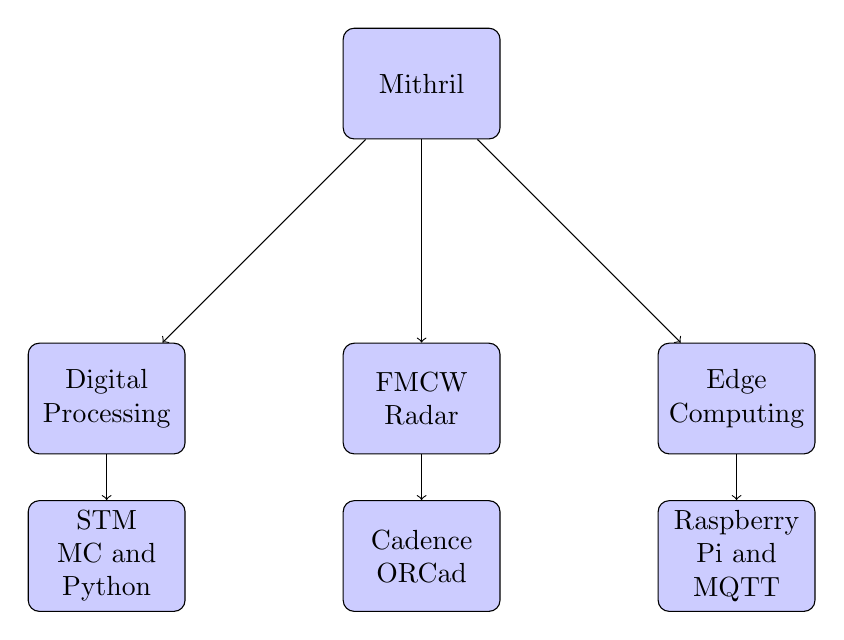
\begin{tikzpicture}[node distance = 2cm, auto]
      % Define block styles
      \tikzstyle{block} = [rectangle, draw, fill=blue!20, 
          text width=5em, text centered, rounded corners, minimum height=4em]
      \tikzstyle{line} = [draw, ->]
  
      % Place nodes
      \node [block] (mithril) {Mithril};
      \node [block, below of=mithril, node distance=4cm] (radar) {FMCW Radar};
      \node [block, left of=radar, node distance=4cm] (processing) {Digital Processing};
      \node [block, right of=radar, node distance=4cm] (networking) {Edge Computing};
      \node [block, below of=processing, node distance=2cm] (STM) {STM MC and Python};
      \node [block, below of=radar, node distance=2cm] (ORCad) {Cadence ORCad};
      \node [block, below of=networking, node distance=2cm] (pi) {Raspberry Pi and MQTT};
      % Draw edges
      \path [line] (mithril) -- (radar);
      \path [line] (mithril) -- (processing);
      \path [line] (mithril) -- (networking);
      \path [line] (radar) -- (ORCad);
      \path [line] (processing) -- (STM);
      \path [line] (networking) -- (pi);
  \end{tikzpicture}
  \caption{Flowchart of the Mithril system}
  \label{fig:mithril_flowchart}
  \end{figure}
Mithril is a nodal FMCW radar system that incorporates traditional FMCW radar,
digital processing, edge computing, and distributed networking. The initial application of this project was for a military context.
State of the art missile defense systems cost too much and are too big to be viable in many places, and while our system doesn't compare to
systems like the Iron Dome or Patriot System it could allow for at least an alert for civilians to leave possible shelling and bombing sites.
The system would include small radar nodes capable of detecting missiles and electronically steering their line of sight via phased array antennas.
Multiple nodes could work in tandem to communicate their findings, allowing for a wider range of sight and active tracking of projectiles. The network would
be able to function regardless of how many nodes there were, and still continue to function if nodes are destroyed.

As can be seen in Figure \ref{fig:mithril_flowchart},
the radar was designed as a standalone PCB in ORCad, digital processing was handled by
STM microcontrollers, and distributed networking is done via Raspberry Pi's and the MQTT protocol.
All of these components were designed, engineered, and interfaced from scratch with a limited budget
of 2000 dollars.

\section{FMCW Radar PCB}
\begin{figure}[H]
  \centering
  \scalebox{.11}{\includegraphics{ProjectImages/pcb_1.jpg}}
\caption{Mithril PCB}
\label{img:mithrilPCB_1}
\end{figure}
The heart of the project is a standalone PCB capable of FMCW radar and phased array beamforming, which can be seen in Image \ref{img:mithrilPCB_1}.
The PCB has a transmitting and receiving portion, each with several stages. The TX portion has a stage for signal synthesis,
phase shifting, and amplification. The RX portion has a stage for amplification, mixing, and baseband filtering/amplifying.
There are also GPIO pins for interfacing with the microcontroller, as well as test pins for analyzing the signals we receive.
This was foreign ground for the entire team, and was started by first researching common RF chains, picking parts that could handle
the afformentioned stages, designing the schematic and layout in ORCad, and then printing and assembling the board. Afterwards,
we tested for weeks to find different issues and workarounds which will be mentioned later.

\section{Digital Processing}
The digital processing was handled entirely by the \href{https://www.st.com/en/evaluation-tools/nucleo-f756zg.html}{STM-F756ZG}.
Two of them were used in the final implementation, where one was responsible for generating a ramp voltage which will be discussed
later, and the other responsible for sampling the radar's received signal, windowing the signal, taking the FFT, transmitting 
the FFT over UART, and receiving commands over UART to program the phase shifter on the PCB via its GPIO pins. This was a lot of tasks,
and all of it was programmed to run in a superloop with the help of DMA and interrupts.

\section{Networking}
Mithril relies on the idea of using smaller, cheaper radar PCB nodes which work together to achieve the same sort of capabiltiy as a much larger system. To achieve this PCB radar nodes must be able to communciate with one another and be able to coordinate and send data in a safe and secure manner. Furthermore, the network must be able to easily add new nodes into the system as well as be able to handle if and when nodes are destroyed or if communication becomes impossible. To achieve this we have implemeneted a mesh network topology for our defense system.

A mesh network is a type of network topology in which each node in the network can communicate with multiple other nodes in the network, creating a highly redundant and resilient network architecture. In a mesh network, each node acts as both a sender and a receiver, relaying data through the network until it reaches its intended destination. This allows for the creation of a self-configuring and self-healing network that can be quickly deployed and is resilient to failures. Figure \ref{Figure::Sample Mesh}  shows a typical mesh network configuration.


\begin{figure}[H]
  \centering
  \scalebox{0.5}{\includegraphics{Figures/Sample_mesh.jpg}}
  \caption{\label{Figure::Sample Mesh} Sample Mesh Network Configuration}
  \end{figure}

  Mesh networks have numerous applications, and one of the most promising is for Internet of Things (IoT) devices. IoT devices typically rely on wireless communication, but traditional wireless networks may not be sufficient for large-scale deployments. An ad-hoc mesh network can provide the necessary scalability and reliability for IoT devices, allowing them to communicate with each other and with central servers without relying on a single point of failure. This makes them ideal for scenarios where traditional networks may not be available or feasible, such as in disaster response situations or in remote locations both possible locations where Mithril might be employed.

  To actually implement the mesh network we will use Raspberry Pi's to handle all the software and wireless connectivity capabilities. Raspberry Pi's are small, low-cost, single-board computers which provide incredible performance despite their small size and cost. Raspberry Pi's are roughly the size of a credit card and come with various input and output ports, including HDMI, USB, Ethernet, and GPIO (General Purpose Input/Output) pins. They can run a variety of operating systems, including Linux-based distributions such as Raspbian and Ubuntu, and can be programmed in various programming languages, including Python, C, and Java. Because of their small size, low power consumption, and versatility, Raspberry Pi's are an excellent platform for the creation of low-cost and flexible ad-hoc mesh networks. Mithril will utilize a series of Raspberry Pi's along with some USB Wi-Fi dongles to implement an ad-hoc network which will trasmit radar data. Mithril achieves this this by utilizing several Linux software libraries together to create a framework for a Raspberry-Pi enabled mesh network.

